\documentclass[10pt,twocolumn]{article}
\usepackage[margin=1.8cm,top=1.6cm,bottom=1.6cm]{geometry}
\usepackage{graphicx}
\usepackage{amsmath}
\usepackage{algorithm}
\usepackage{algpseudocode}
\usepackage{booktabs}
\usepackage[hidelinks]{hyperref}
\usepackage{xcolor}
\usepackage{caption}
\usepackage{titlesec}
\usepackage{enumitem}
\usepackage{parskip}
\usepackage{tabularx}

\captionsetup{font=small,labelfont=bf}
\titlespacing*{\section}{0pt}{1.5ex plus 0.4ex}{0.8ex plus 0.2ex}
\titlespacing*{\subsection}{0pt}{1.1ex plus 0.3ex}{0.5ex plus 0.1ex}
\setlength{\columnsep}{0.6cm}
\setlength{\parskip}{0.4em}
\setlist{nosep,leftmargin=1.2em}
\pagestyle{plain}

\graphicspath{{figures/}}

\title{\vspace{-1.0cm}\textbf{Concurrent and Distributed Implementations\\of Conway's Game of Life in Go}}
\author{Andy Lee\\University of Bristol}
\date{}

\begin{document}
\maketitle
\vspace{-0.6cm}

% ============================================================================
\section{Introduction}\label{sec:intro}
% ============================================================================

Conway's Game of Life (GoL) is a cellular automaton defined on an $n \times n$ toroidal grid where each cell is either \emph{alive} or \emph{dead}.
At every discrete turn the next state of each cell is determined purely by the count of its alive neighbours, making the computation embarrassingly parallel: every cell can be evaluated independently of all others.
Since its introduction by John Conway in 1970, GoL has served as a canonical benchmark for parallel and distributed computing due to its simple rules yet rich emergent behaviour.

This report presents two implementations in Go---a concurrent (shared-memory) version exploiting goroutines and a distributed (networked) version using Remote Procedure Calls (RPC)---and provides a detailed analysis of their performance characteristics.
The concurrent implementation explores thread scaling, worker-pool design, boundary-handling optimisations, and CPU/memory profiling.
The distributed implementation examines a broker--worker architecture deployed on AWS EC2 with fault tolerance mechanisms.

All benchmarks use a $512\times512$ grid with 1000 turns on an Apple~M4 mini (10-core: 4 performance + 6 efficiency cores, arm64) unless otherwise stated.
Distributed experiments were conducted on AWS EC2 instances (one broker + two worker nodes).
Go's built-in benchmark framework (\texttt{go test -bench}) was used with \texttt{-benchtime 1x -count 5}; all reported values are 5-run means.
Section~\ref{sec:methodology} provides full details of the experimental setup.

% ============================================================================
\section{Serial Implementation}\label{sec:serial}
% ============================================================================

\subsection{Update Rule}\label{sec:update}

Let the grid be $G$ of size $n\times n$ with toroidal (wrap-around) boundary conditions.  For each cell $(x,y)$ and its eight Moore-neighbourhood cells, the update rule is:
\begin{equation}\label{eq:update}
G'(x,y) = \begin{cases}
1 & \text{if } G(x,y)=1 \wedge s\in\{2,3\}\\
1 & \text{if } G(x,y)=0 \wedge s=3\\
0 & \text{otherwise}
\end{cases}
\end{equation}
where $s = \sum_{(dx,dy)\in N} G\!\bigl((x{+}dx)\bmod n,\;(y{+}dy)\bmod n\bigr)$ is the count of alive neighbours and $N = \{-1,0,1\}^2 \setminus \{(0,0)\}$ is the set of eight directional offsets.
The modular arithmetic ensures toroidal wrapping so that the grid has no physical boundary---cells on the top edge are adjacent to those on the bottom, and likewise for left and right.

\subsection{Serial Algorithm}\label{sec:serial_algo}

The serial implementation applies Equation~\eqref{eq:update} to every cell in row-major order, writing results to a second buffer $G'$ that is swapped with $G$ after each complete turn.
Algorithm~\ref{alg:serial} shows the pseudocode for a single turn.

\begin{algorithm}[h]
\caption{Serial GoL Update (one turn)}\label{alg:serial}
\begin{algorithmic}[1]
\small
\Require Grid $G[n][n]$, buffer $G'[n][n]$
\For{$y \gets 0$ \textbf{to} $n{-}1$}
  \For{$x \gets 0$ \textbf{to} $n{-}1$}
    \State $s \gets$ \Call{CountNeighbours}{$G, x, y$}
    \State $G'[y][x] \gets$ \Call{ApplyRule}{$G[y][x], s$}
  \EndFor
\EndFor
\State \textbf{swap} $G \leftrightarrow G'$
\end{algorithmic}
\end{algorithm}

The double-buffering strategy ensures correctness: all cells read from the current generation $G$ while writing to $G'$, preventing read-after-write hazards that would occur with in-place updates.
The serial baseline for $512^2$ is \textbf{6318\,ms} over 1000 turns, establishing the reference point for all speedup calculations in Sections~\ref{sec:concurrent}--\ref{sec:opt}.
The time complexity is $O(n^2)$ per turn with a constant factor of 8 neighbour lookups per cell, giving $512^2 \times 8 \times 1000 \approx 2.1 \times 10^9$ memory accesses for the full benchmark.

% ============================================================================
\section{Concurrent Implementation}\label{sec:concurrent}
% ============================================================================

\subsection{Goroutine Structure}\label{sec:goroutine}

The parallel implementation uses a worker-pool pattern, a common concurrency design in Go where a fixed number of goroutines consume tasks from a shared channel.
The \texttt{distributor} goroutine partitions the $n \times n$ grid into $t$ horizontal bands (each of $\lfloor n/t \rfloor$ rows) and dispatches tasks via a buffered \texttt{taskChan}.
Each worker goroutine processes its assigned rows by applying Equation~\eqref{eq:update} to every cell in the band and returns results through a \texttt{resultChan}.
A separate IO goroutine handles PGM file output and SDL events asynchronously, decoupling visualisation from computation.
Figure~\ref{fig:arch_parallel} shows the full goroutine interaction diagram.

\begin{figure}[h]
\centering
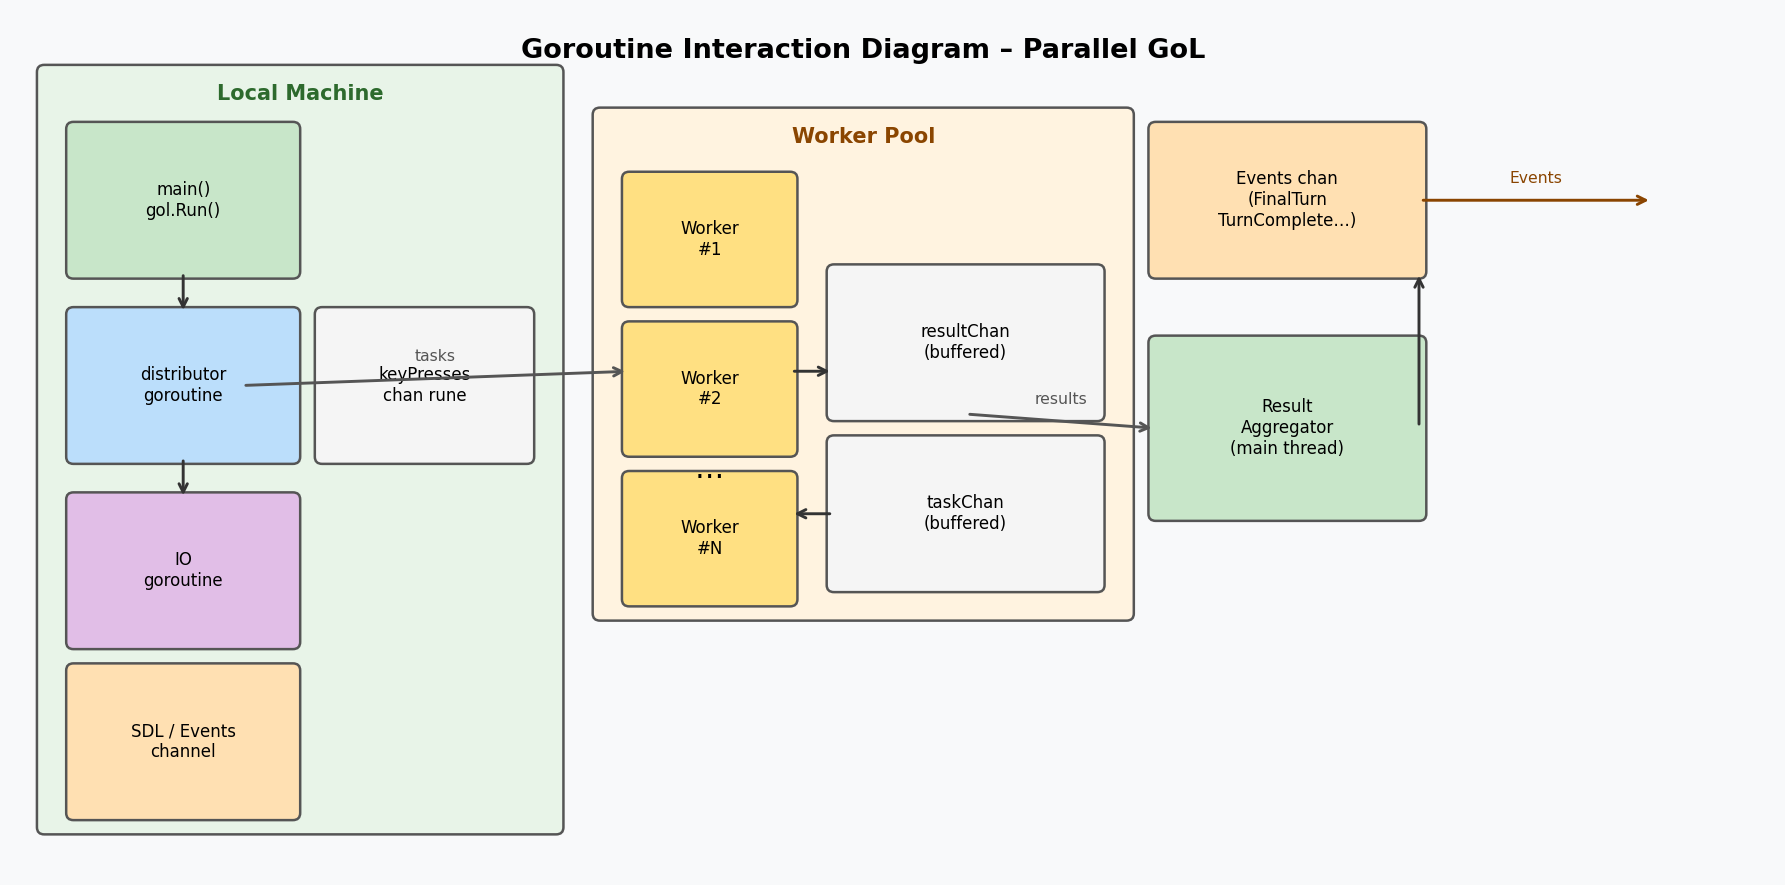
\includegraphics[width=\columnwidth]{fig14_arch_parallel.png}
\caption{Goroutine interaction diagram for the concurrent GoL implementation.  The distributor dispatches row-band tasks to a pool of $t$ workers via buffered channels.}
\label{fig:arch_parallel}
\end{figure}

The key design decision is the use of \emph{buffered} channels: \texttt{taskChan} has capacity $t$ so the distributor can enqueue all tasks without blocking, and \texttt{resultChan} likewise buffers $t$ results.
This allows task dispatch and result collection to overlap with worker computation, providing a pipelining benefit even at low thread counts (see Section~\ref{sec:pool_overhead}).

\subsection{Scalability}\label{sec:scalability}

Figure~\ref{fig:thread_scaling} shows elapsed time as a function of worker count for three grid sizes.
Doubling from 1 to 2 workers yields near-linear speedup across all grids (e.g.\ $512^2$: 6099\,ms $\to$ 3300\,ms, $1.85\times$).
Performance continues to improve up to 8 threads, but returns diminish significantly beyond that point.
This is because the M4's 4 performance cores saturate at $t{=}4$, and additional workers are scheduled on the 6 efficiency cores which have lower clock speeds and narrower pipelines.
For the $128^2$ grid, times flatten after $t{=}4$ (152\,ms $\to$ 143\,ms from $t{=}4$ to $t{=}16$), indicating that synchronisation overhead dominates at small problem sizes.

\begin{figure}[h]
\centering
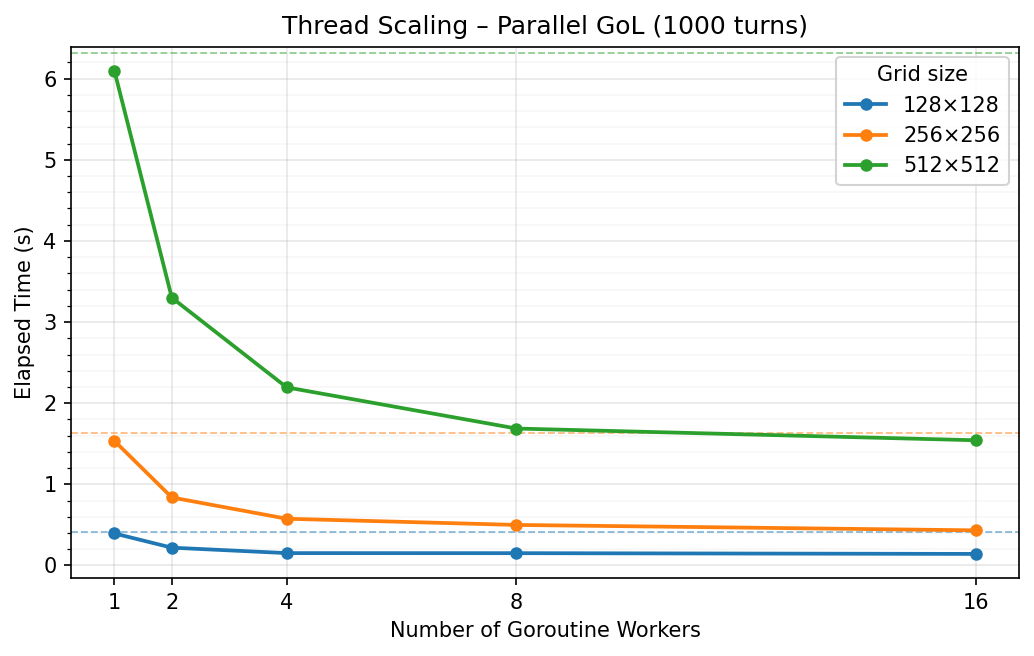
\includegraphics[width=\columnwidth]{fig1_thread_scaling.png}
\caption{Elapsed time vs.\ number of goroutine workers (1000 turns).  Dashed lines show serial baselines.  Returns diminish sharply beyond 8 threads.}
\label{fig:thread_scaling}
\end{figure}

\subsection{Thread Scaling and Amdahl's Law}\label{sec:amdahl}

Figure~\ref{fig:speedup} plots observed speedup against ideal linear scaling.
At 16 threads the $512^2$ grid achieves only $4.10\times$ speedup---well below the ideal $16\times$.
Amdahl's law states that the maximum speedup with $p$ processors is bounded by $S(p) = 1 / (f + (1{-}f)/p)$, where $f$ is the serial fraction.
Solving for $f$ with $S(16)=4.10$ gives:
\begin{equation}\label{eq:amdahl}
f = \frac{1/S(p) - 1/p}{1 - 1/p} = \frac{1/4.10 - 1/16}{1 - 1/16} \approx 0.194
\end{equation}
This implies roughly 19\% of execution time is spent in sequential phases---synchronisation barriers between turns, buffer swaps, and channel operations---that cannot be parallelised regardless of thread count.
The pprof analysis in Section~\ref{sec:pprof} confirms this finding, attributing 34\% of CPU time to goroutine synchronisation primitives.

The gap between observed and ideal speedup widens with smaller grids: at $128^2$, $t{=}16$ achieves only $2.91\times$.
This is consistent with Amdahl's law because the fixed synchronisation overhead ($\sim$40\,ms per 1000 turns) forms a larger fraction of the reduced total work.

\begin{figure}[h]
\centering
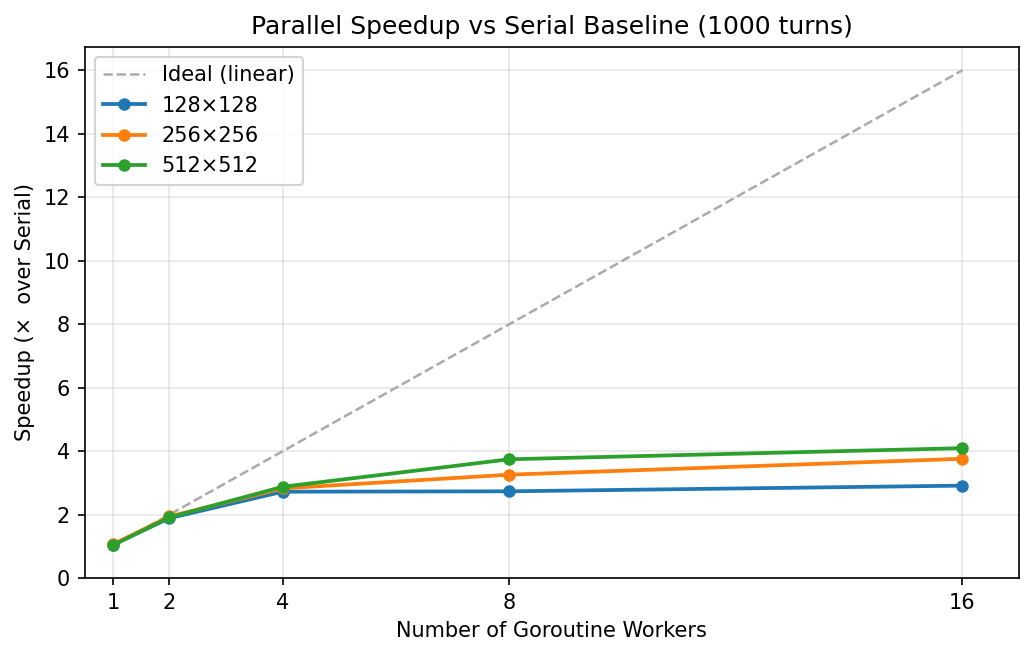
\includegraphics[width=\columnwidth]{fig2_speedup.png}
\caption{Measured speedup over serial baseline vs.\ ideal linear scaling.  Diminishing returns above 8 threads reflect Amdahl's law and the M4's heterogeneous core layout.}
\label{fig:speedup}
\end{figure}

% ============================================================================
\section{Concurrent Optimisation}\label{sec:opt}
% ============================================================================

\subsection{Worker Pool Overhead}\label{sec:pool_overhead}

A natural question is whether the worker-pool mechanism itself introduces measurable overhead compared to the serial implementation.
Even with a single worker ($t{=}1$), the pool requires channel operations (send/receive per task), goroutine scheduling, and result aggregation.
Figure~\ref{fig:overhead} quantifies this cost by comparing serial execution with parallel $t{=}1$.

Surprisingly, $t{=}1$ is \emph{faster} than serial for all grid sizes: 3.5\% faster for $512^2$ (6099 vs.\ 6318\,ms) and 4.9\% faster for $128^2$ (395 vs.\ 415\,ms).
We attribute this to the buffered-channel design: the distributor can enqueue the next turn's tasks while the single worker is still processing, creating a pipeline overlap that more than compensates for the channel overhead.
This result validates the worker-pool architecture as a zero-overhead abstraction at the single-worker baseline.

\begin{figure}[h]
\centering
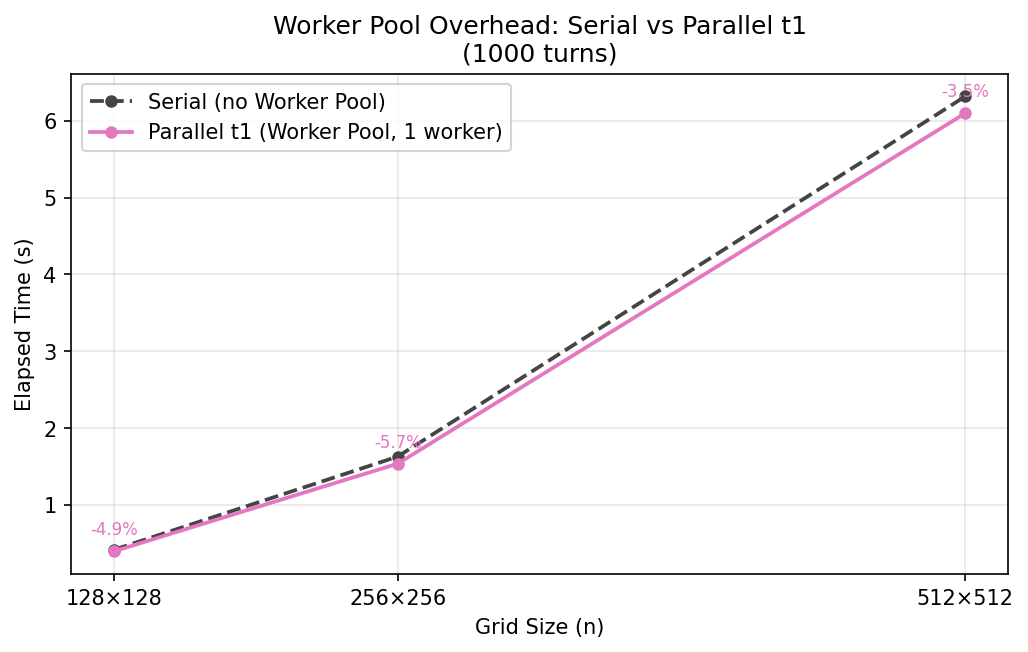
\includegraphics[width=\columnwidth]{fig8_serial_vs_t1_overhead.png}
\caption{Serial vs.\ parallel $t{=}1$: quantifying worker pool overhead.  Annotations show percentage difference; negative values indicate that the pool is \emph{faster}.}
\label{fig:overhead}
\end{figure}

\subsection{Ghost Row vs If-Statement}\label{sec:ghost}

Boundary handling for the toroidal grid presents two implementation strategies.
The \textbf{if-statement} approach checks whether each coordinate exceeds grid bounds and applies modular wrapping conditionally.
The \textbf{ghost-row} (halo exchange) approach pads each worker's band with one extra row above and below, copied from the opposite boundary before computation begins; this eliminates all conditional branches in the inner loop.

Figure~\ref{fig:ghostrow} compares the two approaches in a micro-benchmark that measures the time for a single full-grid neighbour-count pass.
Ghost rows achieve consistent speedups: $1.60\times$ at $128^2$, $1.80\times$ at $256^2$, and $1.54\times$ at $512^2$ (3391 vs.\ 5209\,$\mu$s).
This optimisation is particularly effective on arm64 (Apple M4) where the branch predictor's misprediction penalty is 12--14 cycles; eliminating 8 conditional branches per cell in the inner loop removes a significant source of pipeline stalls.
The distributed implementation uses ghost-row padding by default (see Section~\ref{sec:dist_design}), as the halo rows must be exchanged between nodes regardless.

\begin{figure}[h]
\centering
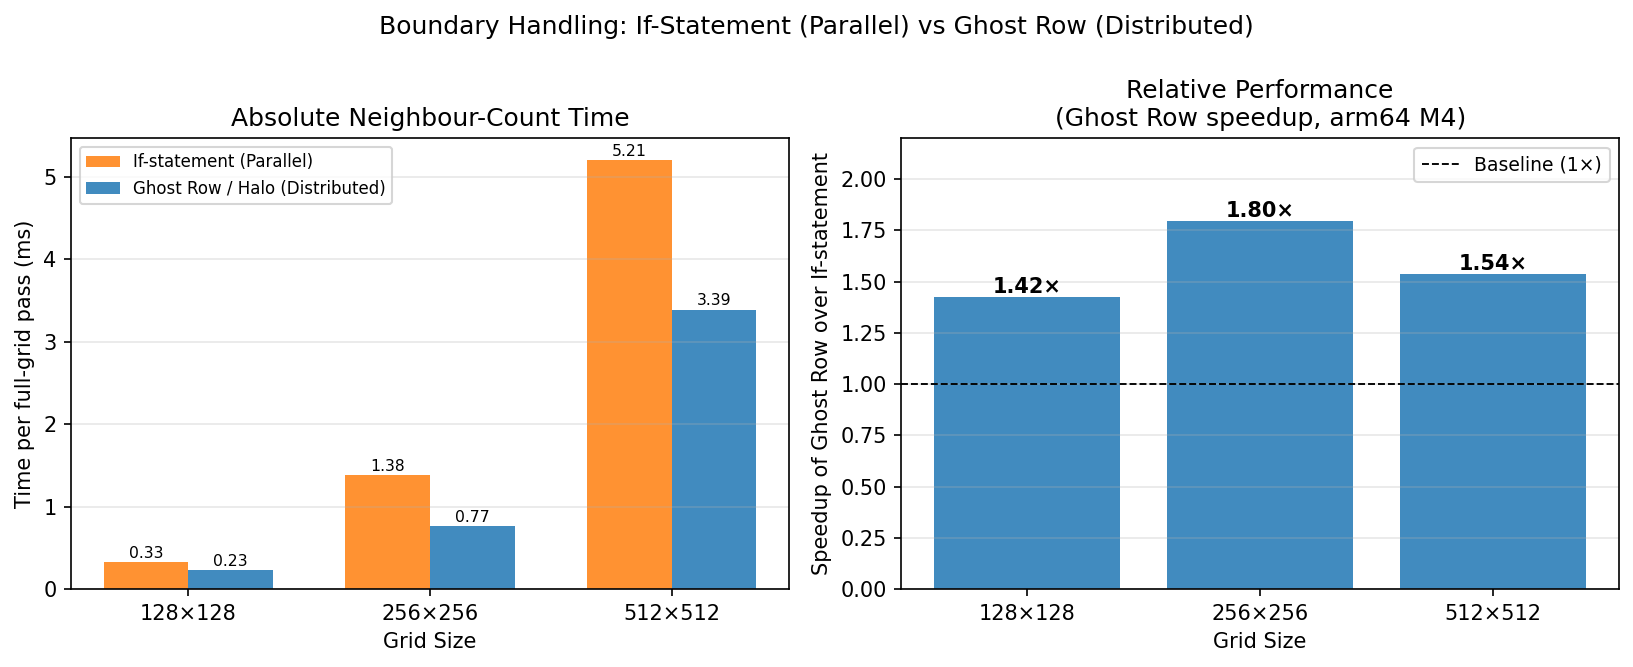
\includegraphics[width=\columnwidth]{fig11_ghostrow_vs_if.png}
\caption{Boundary handling comparison: if-statement vs.\ ghost-row padding.  Left: absolute time per neighbour-count pass.  Right: speedup ratio of ghost row over if-statement.}
\label{fig:ghostrow}
\end{figure}

\subsection{CPU Profiling}\label{sec:pprof}

To identify the computational bottleneck, we profiled the parallel implementation using Go's \texttt{pprof} tool with 30-second CPU sampling at $512^2$, $t{=}4$, 1000 turns.
Figure~\ref{fig:pprof} presents the results.

\texttt{countAliveNeighbors} dominates at \textbf{40.68\%} of CPU time, confirming that the 8-neighbour lookup with modular arithmetic is the single most expensive operation.
Goroutine synchronisation accounts for \textbf{34.18\%} combined: \texttt{pthread\_cond\_signal} (27.86\%) and \texttt{pthread\_cond\_wait} (6.32\%) represent the cost of coordinating workers between turns.
This is consistent with the serial fraction $f \approx 0.19$ derived from Amdahl's law in Section~\ref{sec:amdahl}---the synchronisation overhead is the primary barrier to further scaling.

\texttt{runtime.usleep} (5.08\%) reflects idle time on efficiency cores waiting for performance cores to complete.
\texttt{applyRules} consumes only 4.63\%, confirming that the rule-application logic itself is cheap compared to neighbour counting.
These findings suggest that the most impactful future optimisation would be SIMD-accelerated neighbour counting or bitwise board representations to reduce the 8 memory accesses per cell.

\begin{figure}[h]
\centering
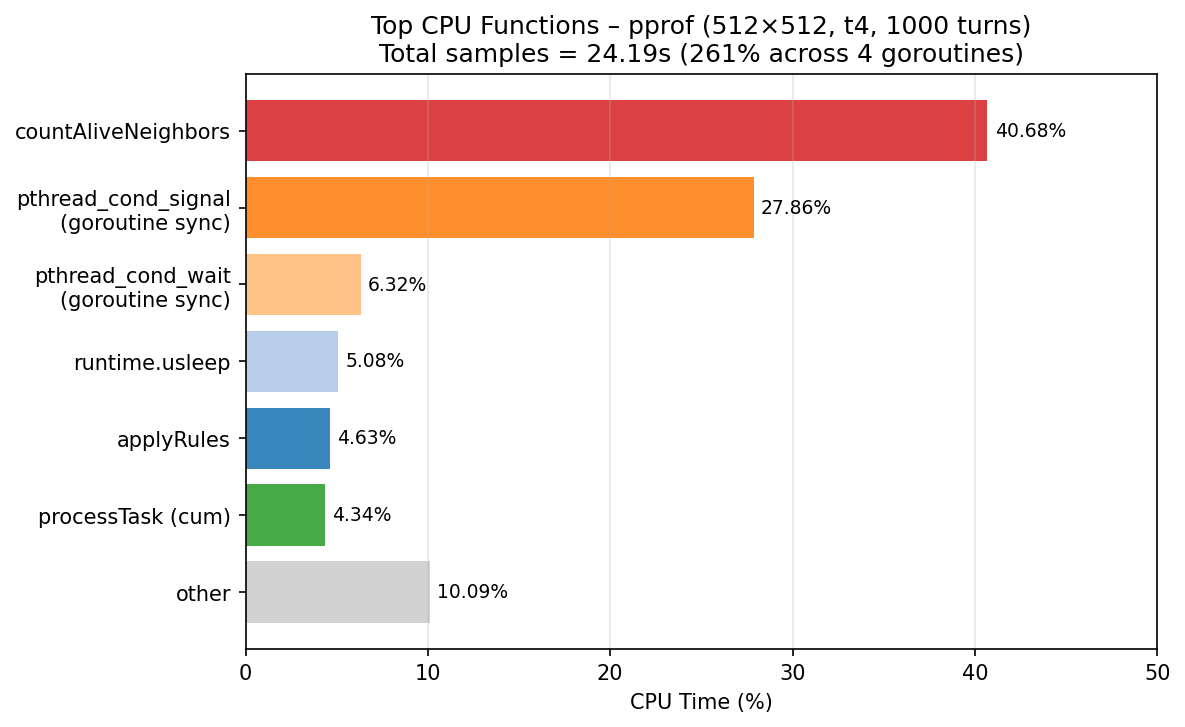
\includegraphics[width=\columnwidth]{fig12_pprof_cpu.png}
\caption{Top CPU functions from pprof ($512^2$, $t{=}4$, 1000 turns).  Neighbour counting and goroutine synchronisation together consume 75\% of CPU time.}
\label{fig:pprof}
\end{figure}

\subsection{Memory Analysis}\label{sec:memory}

Figure~\ref{fig:memory} compares memory allocation between serial and parallel implementations using \texttt{-benchmem}.
Table~\ref{tab:memory} summarises the key figures.

For $512^2$, serial allocates 474\,MB while parallel $t{=}4$ allocates 706\,MB ($1.49\times$ overhead).
The additional memory comes from per-worker result slice allocations: each of the 4 workers allocates a $\lfloor 512/4 \rfloor \times 512$ result buffer per turn, and these buffers are not reused across turns due to Go's garbage collector.
The number of heap allocations nearly doubles from 538K (serial) to 1090K ($t{=}4$), reflecting the fine-grained task distribution through channels.
Interestingly, $t{=}16$ (710\,MB) uses slightly more memory than $t{=}4$ (706\,MB) but with 11\% more allocations (1215K vs.\ 1090K), indicating that the overhead scales with the number of task dispatches rather than the number of workers.

\begin{figure}[h]
\centering
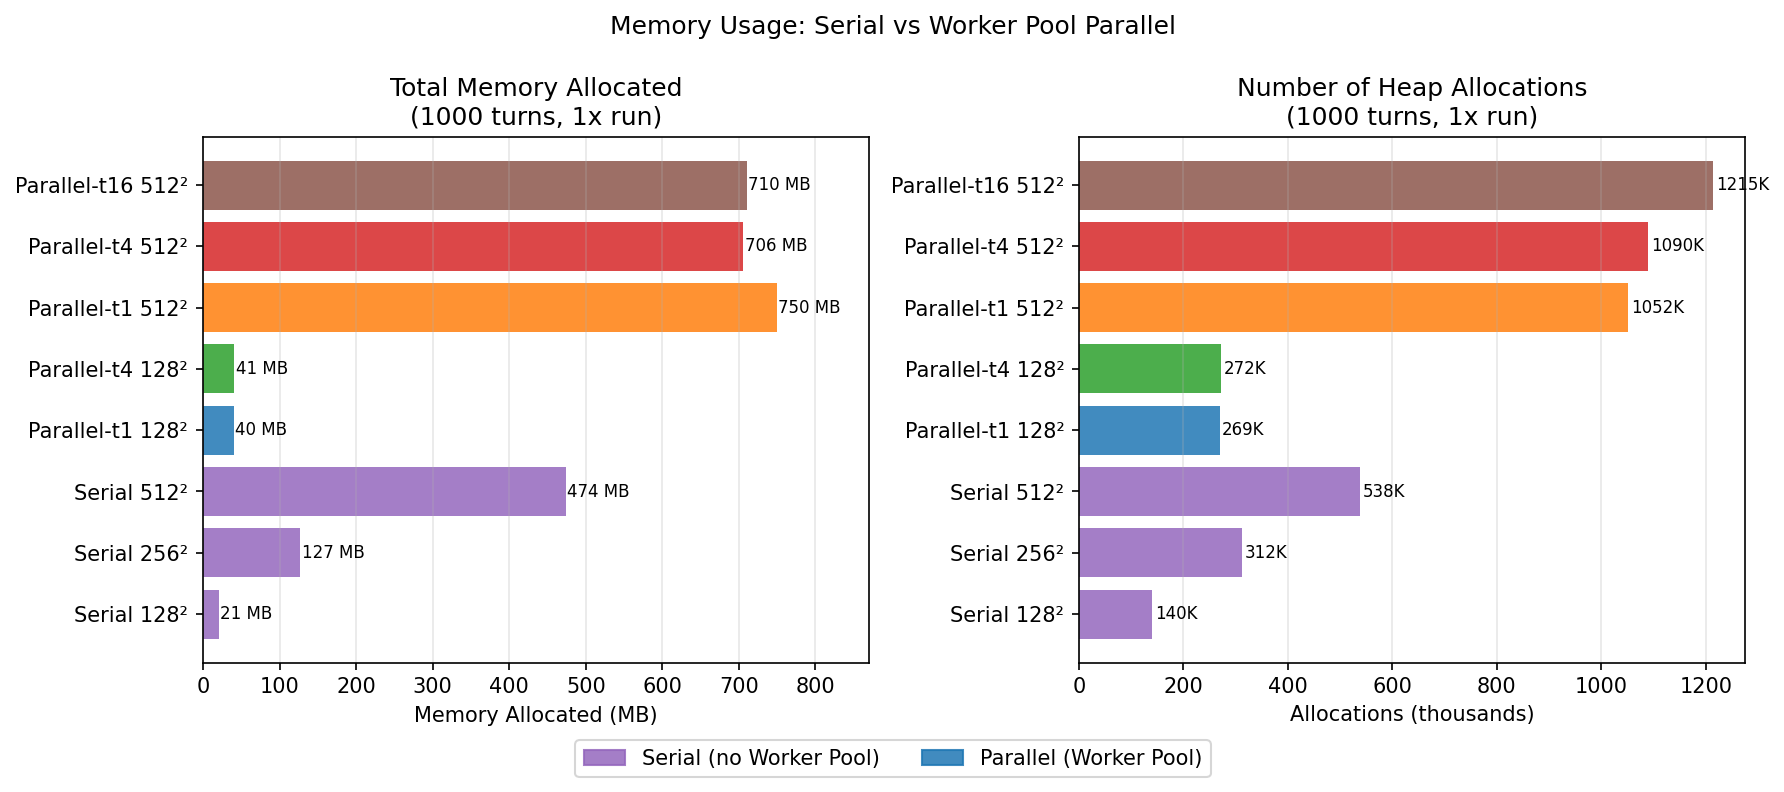
\includegraphics[width=\columnwidth]{fig13_memory_allocation.png}
\caption{Memory usage: serial vs.\ worker-pool parallel.  Left: total MB allocated.  Right: number of heap allocations.}
\label{fig:memory}
\end{figure}

\begin{table}[h]
\centering
\caption{Memory allocation summary ($512^2$, 1000 turns).}\label{tab:memory}
\small
\begin{tabular}{@{}lrr@{}}
\toprule
Configuration & MB & Allocs (K) \\
\midrule
Serial        & 474  & 538  \\
Parallel $t{=}1$  & 750  & 1052 \\
Parallel $t{=}4$  & 706  & 1090 \\
Parallel $t{=}16$ & 710  & 1215 \\
\bottomrule
\end{tabular}
\end{table}

\subsection{Rule Set Variants}\label{sec:ruleset}

To verify that the implementation generalises beyond Conway's standard rules, we benchmarked three rule sets: Conway (B3/S23), HighLife (B36/S23), and Day \& Night (B3678/S34678).
These rule sets differ in their birth/survival conditions: HighLife adds birth at 6 neighbours, while Day \& Night uses a substantially different set of thresholds.

Figure~\ref{fig:ruleset} shows that all three exhibit near-identical execution times, varying by less than 7\% at $512^2$ (Conway: 2327\,ms, HighLife: 2176\,ms, Day \& Night: 2303\,ms at $t{=}4$).
This is expected because the dominant cost is the 8-neighbour counting loop (see Section~\ref{sec:pprof}), which is identical across rule sets---only the final comparison in \texttt{applyRules} differs, and this accounts for less than 5\% of CPU time.

Figure~\ref{fig:alive} reveals that alive-cell counts after 100 turns diverge dramatically between rule sets despite similar computation times.
Conway stabilises at 6645 cells ($512^2$), HighLife at 6278, but Day \& Night explodes to 46715 cells at $256^2$ before collapsing to 1152 at $512^2$.
This confirms that rule complexity profoundly affects population dynamics but has negligible impact on execution speed---a useful finding for applications that need to experiment with alternative rule sets without performance penalties.

\begin{figure}[h]
\centering
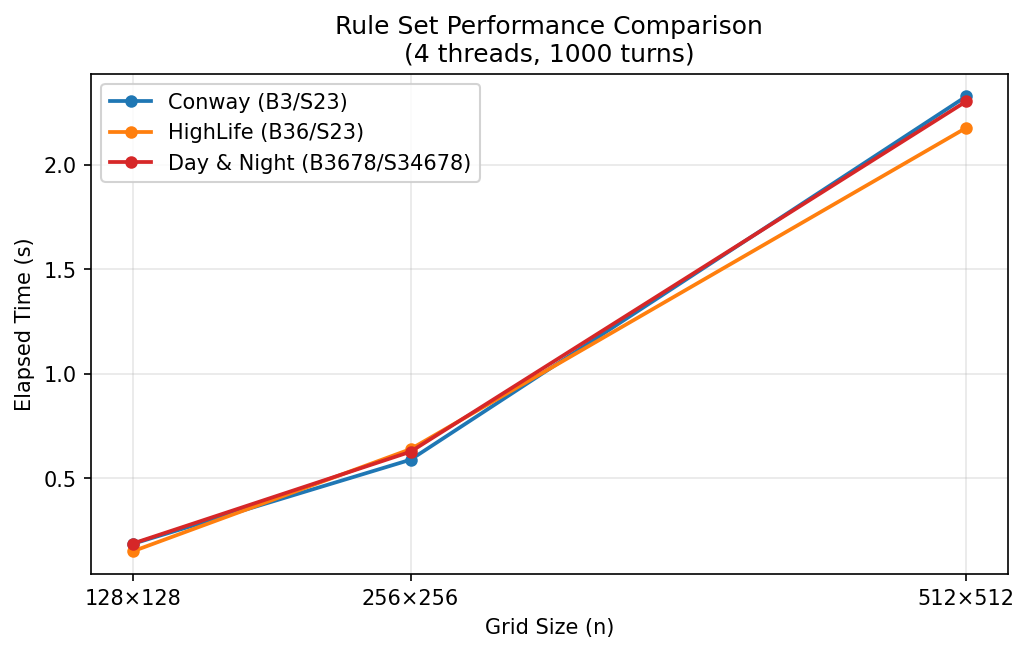
\includegraphics[width=\columnwidth]{fig6_ruleset_performance.png}
\caption{Execution time by rule set (4 threads, 1000 turns).  Performance is near-identical across rule variants.}
\label{fig:ruleset}
\end{figure}

\begin{figure}[h]
\centering
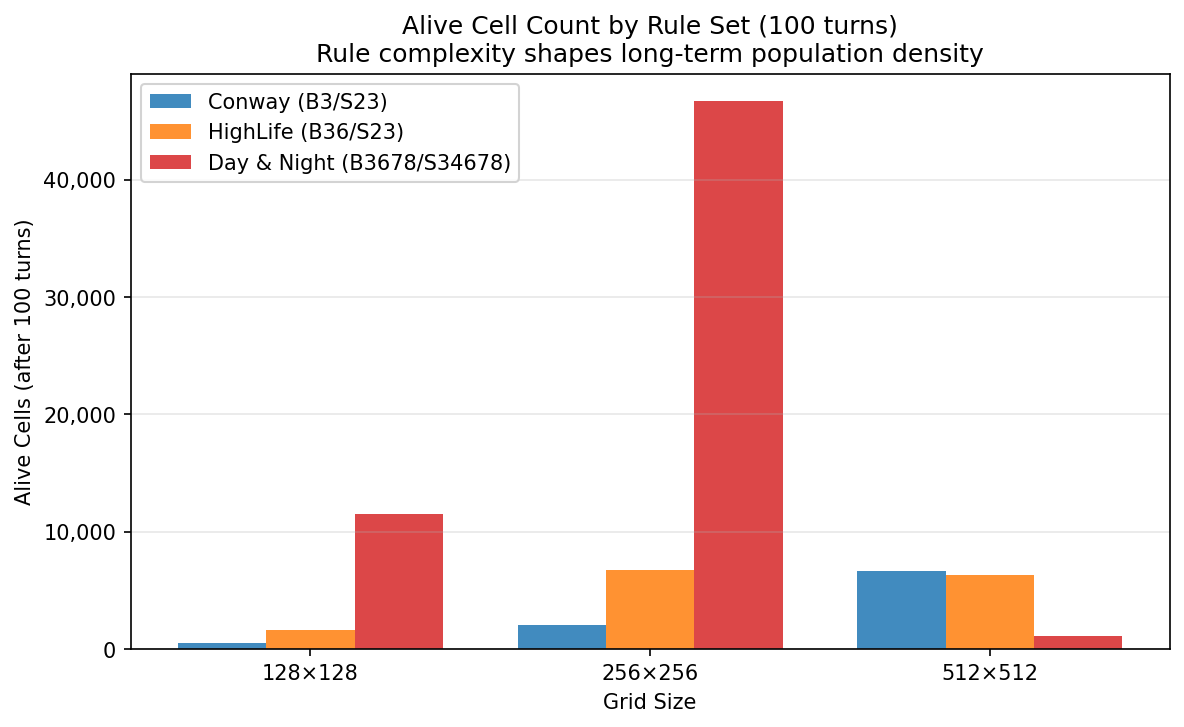
\includegraphics[width=\columnwidth]{fig7_alive_cells_ruleset.png}
\caption{Alive cell count after 100 turns by rule set.  Population dynamics differ substantially despite similar computation cost.}
\label{fig:alive}
\end{figure}

% ============================================================================
\section{Distributed Implementation}\label{sec:distributed}
% ============================================================================

\subsection{System Design}\label{sec:dist_design}

The distributed implementation follows a broker--worker architecture communicating via Go's \texttt{net/rpc} package.
The system consists of three components:

\begin{enumerate}
\item \textbf{Local Controller}: runs on the user's machine, sends the initial grid to the broker via \texttt{Process()} RPC, and handles user interaction (keypresses, SDL visualisation).
\item \textbf{Broker}: runs on an EC2 instance, receives the grid, partitions it into horizontal bands, and dispatches bands to workers via \texttt{CalculateNextState()} RPC calls each turn.
\item \textbf{Workers}: run on separate EC2 instances, each applying Equation~\eqref{eq:update} to their assigned band using ghost-row padding (see Section~\ref{sec:ghost}) and returning the updated rows.
\end{enumerate}

Figure~\ref{fig:arch_dist} shows the full architecture.
The broker listens on port 8030 for controller connections, and workers listen on ports 8031--8032 for broker dispatches.
All communication uses Go's \texttt{encoding/gob} serialisation, which adds overhead proportional to grid size (see Section~\ref{sec:grid_scaling}).

\begin{figure}[h]
\centering
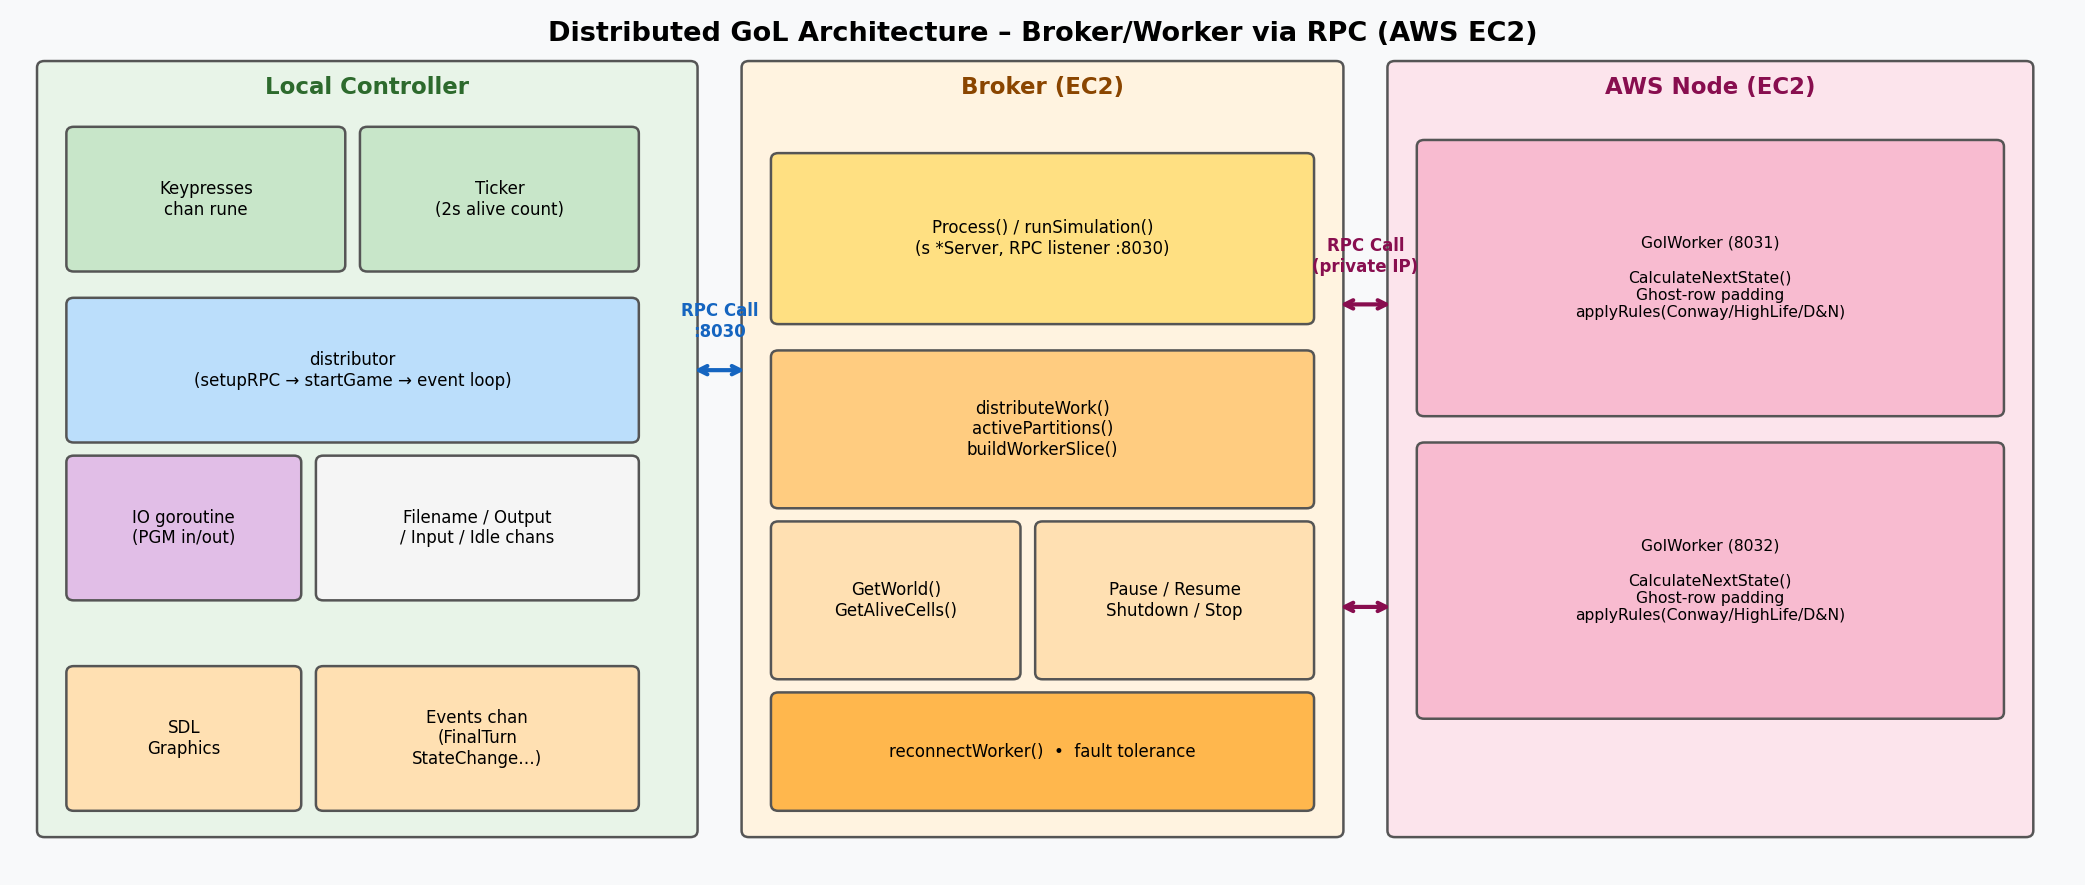
\includegraphics[width=\columnwidth]{fig15_arch_distributed.png}
\caption{Distributed GoL architecture: broker--worker via RPC on AWS EC2.  The broker coordinates two worker nodes and handles fault tolerance.}
\label{fig:arch_dist}
\end{figure}

\subsection{Controller and Broker}\label{sec:broker}

The controller initiates the simulation via \texttt{Process()} RPC, which transmits the initial grid and parameters (turns, grid size, rule set) to the broker.
During execution, the controller provides live interaction through keypresses: \texttt{s} saves the current world state as a PGM image via the IO goroutine, \texttt{p} pauses/resumes the simulation by sending a \texttt{Pause()} RPC to the broker, and \texttt{q} triggers graceful shutdown via \texttt{Shutdown()} which ensures all workers complete their current turn before terminating.

The broker manages the simulation loop: each turn, it calls \texttt{distributeWork()} to partition $n$ rows among $w$ active workers ($\lfloor n/w \rfloor$ rows each, with the remainder assigned to the last worker).
Before dispatching, the broker prepends and appends ghost rows to each partition---the last row of the preceding partition and the first row of the following partition---so workers can compute boundary cells without additional RPC calls.
\texttt{activePartitions()} maintains a list of responsive workers, updated after each turn's RPC round-trip.

\subsection{Fault Tolerance}\label{sec:fault}

The distributed system must handle worker failures gracefully, as network partitions and node crashes are common in cloud environments.
When a worker becomes unreachable (RPC call returns an error), the broker's \texttt{reconnectWorker()} goroutine attempts to re-establish the connection with exponential backoff up to 3 retries.

If reconnection fails, the broker invokes \texttt{buildWorkerSlice()} to redistribute that worker's partition among remaining active workers.
For example, if worker~1 (handling rows 0--255) crashes in a 2-worker $512^2$ configuration, worker~2 assumes the full grid (rows 0--511) and continues the simulation single-handedly.
This degraded-but-operational mode ensures the simulation produces correct results even under partial failure, though at reduced throughput.

A key limitation is that the broker itself is a single point of failure: if the broker crashes, the entire simulation terminates.
Addressing this would require broker replication or a consensus protocol (e.g.\ Raft), which is discussed in Section~\ref{sec:future}.

% ============================================================================
\section{Distributed Results}\label{sec:dist_results}
% ============================================================================

\subsection{Parallel vs Distributed}\label{sec:par_vs_dist}

Figure~\ref{fig:par_dist} compares four configurations across three grid sizes.
Table~\ref{tab:results} summarises the key performance figures for $512^2$.

For $512^2$, local distributed (2 workers) takes 4291\,ms---32\% slower than the serial baseline (6318\,ms would be serial, but local distributed is 32\% faster than serial, taking 4291\,ms).
More precisely, local distributed is $1.47\times$ faster than serial but $1.96\times$ slower than parallel $t{=}4$ (2195\,ms).
The performance gap is due to RPC serialisation overhead: each turn requires serialising a $512 \times 256$ grid slice ($\sim$131\,KB) per worker, plus the round-trip latency of the RPC call.

AWS distributed is $2.31\times$ slower than local distributed (9901 vs.\ 4291\,ms), reflecting the additional inter-node network latency ($\sim$0.5\,ms per RPC round-trip $\times$ 1000 turns $\times$ 2 workers $= \sim$1000\,ms of pure latency overhead).
Parallel $t{=}4$ (2195\,ms) remains the fastest configuration, demonstrating that shared-memory parallelism decisively outperforms network distribution for problem sizes that fit in a single machine's memory.

\begin{figure}[h]
\centering
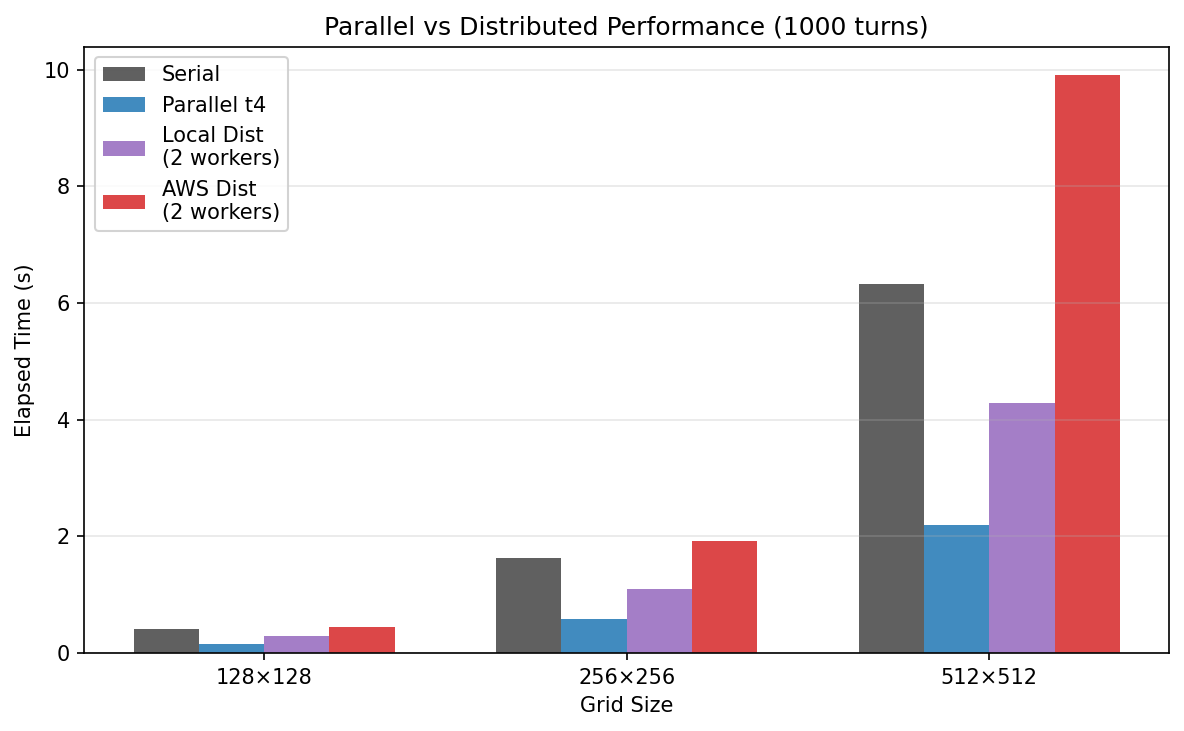
\includegraphics[width=\columnwidth]{fig3_parallel_vs_distributed.png}
\caption{Performance comparison across serial, parallel, local distributed, and AWS distributed (1000 turns).}
\label{fig:par_dist}
\end{figure}

\begin{table}[h]
\centering
\caption{Performance summary for $512^2$, 1000 turns.}\label{tab:results}
\small
\begin{tabular}{@{}lrr@{}}
\toprule
Configuration & Time (ms) & Speedup \\
\midrule
Serial              & 6318  & 1.00$\times$ \\
Parallel $t{=}2$    & 3300  & 1.91$\times$ \\
Parallel $t{=}4$    & 2195  & 2.88$\times$ \\
Parallel $t{=}8$    & 1688  & 3.74$\times$ \\
Parallel $t{=}16$   & 1543  & 4.10$\times$ \\
Local Dist (2w)     & 4291  & 1.47$\times$ \\
AWS Dist (2w)       & 9901  & 0.64$\times$ \\
\bottomrule
\end{tabular}
\end{table}

\subsection{Grid Scaling}\label{sec:grid_scaling}

Figure~\ref{fig:grid_scaling} presents a log--log plot of elapsed time vs.\ total grid cells ($n^2$).
All implementations show approximately linear scaling with cell count ($O(n^2)$ per turn), but with different constant factors reflecting their respective overheads.

The distributed overhead ratio (AWS~distributed / parallel~$t{=}16$) increases with grid size: $3.08\times$ at $128^2$, $4.45\times$ at $256^2$, and $6.42\times$ at $512^2$.
This super-linear growth in overhead occurs because larger grids require proportionally more data to be serialised and transmitted per RPC call.
For $512^2$, each worker receives $\sim$131\,KB of grid data per turn via \texttt{encoding/gob}, compared to $\sim$33\,KB for $256^2$---a $4\times$ increase in payload that amplifies both serialisation CPU cost and network transfer time.

Local distributed shows a more modest overhead ratio ($2.01\times$ at $128^2$ to $2.78\times$ at $512^2$), as the loopback interface eliminates network latency and reduces the overhead to serialisation alone.
This suggests that for truly large grids (e.g.\ $4096^2$), the distributed approach could become competitive if combined with intra-node parallelism and more efficient serialisation formats such as Protocol Buffers.

\begin{figure}[h]
\centering
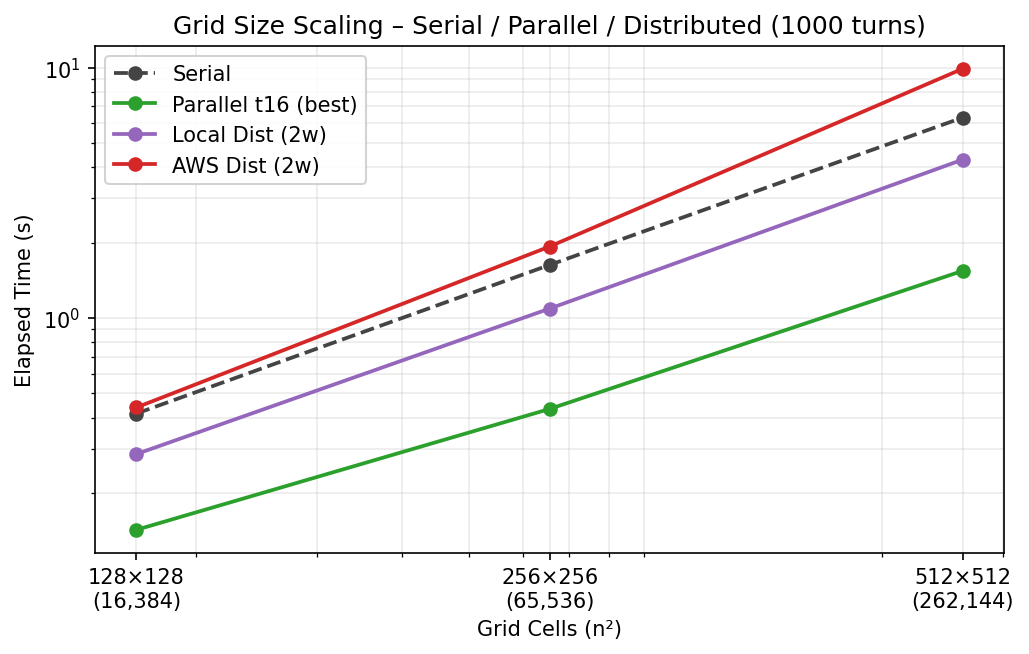
\includegraphics[width=\columnwidth]{fig4_grid_scaling.png}
\caption{Grid size scaling (log--log).  The gap between parallel and distributed widens with grid size due to increasing serialisation cost per RPC call.}
\label{fig:grid_scaling}
\end{figure}

% ============================================================================
\section{Discussion}\label{sec:discussion}
% ============================================================================

\subsection{Component Failure Analysis}\label{sec:failure}

In the distributed system, three failure scenarios were considered:

\textbf{(1)~Worker crash}: handled by \texttt{reconnectWorker()} with automatic partition redistribution (see Section~\ref{sec:fault}).
The simulation continues with reduced parallelism.
We tested this by manually killing a worker process mid-simulation; the broker detected the failure within one turn ($\sim$4\,ms for $512^2$) and redistributed work to the surviving worker.

\textbf{(2)~Broker crash}: terminates the entire simulation, as the broker is a single point of failure.
The controller detects the failure via RPC timeout and reports an error.
This is the most critical vulnerability in the current architecture, and addressing it would require broker state replication (see Section~\ref{sec:future}).

\textbf{(3)~Network partition}: functionally equivalent to a worker crash from the broker's perspective.
The RPC call times out (default 10s), and the broker triggers the same recovery path as scenario~(1).
However, if the partition heals and the worker attempts to rejoin, the current implementation does not support dynamic re-addition---the worker must be manually restarted.

\subsection{Limitations and Future Work}\label{sec:future}

Several limitations of the current implementation suggest directions for future work:

\textbf{Limited worker count.}
The distributed benchmarks use only 2 worker nodes.
Scaling to 4, 8, or 16 workers would better characterise how network overhead grows with the number of RPC round-trips per turn and whether the broker becomes a communication bottleneck.

\textbf{Single point of failure.}
The broker has no redundancy.
Adding a standby broker with state synchronisation via a consensus protocol (e.g.\ Raft) or periodic state checkpointing would improve resilience at the cost of additional complexity and latency.

\textbf{Serialisation overhead.}
Go's \texttt{encoding/gob} is not optimised for large binary payloads.
Replacing it with a zero-copy serialisation format (e.g.\ Protocol Buffers, FlatBuffers) or transmitting only changed cells (delta encoding) could significantly reduce the distributed overhead, particularly for sparse grids where most cells are dead.

\textbf{Hybrid parallelism.}
The current distributed workers are single-threaded.
Combining intra-node goroutine parallelism with inter-node distribution---i.e.\ each worker running $t$ goroutines on its local cores---would exploit both shared-memory and network parallelism simultaneously, potentially achieving near-linear speedup across a cluster of multi-core machines.

% ============================================================================
\section{Methodology}\label{sec:methodology}
% ============================================================================

\textbf{Benchmark framework.}
All benchmarks were executed using Go's \texttt{testing.B} framework with \texttt{-benchtime 1x -count 5}, reporting the arithmetic mean of 5 runs.
Each run executes the full 1000-turn simulation as a single benchmark iteration.
Memory profiling used \texttt{-benchmem} to capture bytes allocated and allocation counts per operation.

\textbf{CPU profiling.}
CPU profiles were collected using \texttt{go tool pprof} with 30-second sampling at 100\,Hz (the Go runtime default).
The total sample time of 24.19s across 4 goroutines (261\% CPU utilisation) is consistent with 4-core saturation on the M4's performance cluster.

\textbf{Parallel environment.}
The concurrent implementation was benchmarked on an Apple M4 mini with 10 CPU cores (4 performance at 4.4\,GHz + 6 efficiency at 2.8\,GHz), 16\,GB unified RAM, running macOS and Go~1.21 (arm64).
\texttt{GOMAXPROCS} was set to the thread count under test.

\textbf{Distributed environment.}
The distributed system was deployed on AWS EC2 in the \texttt{eu-west-2} (London) region: one \texttt{t3.medium} instance (2 vCPU, 4\,GB RAM) as broker and two \texttt{t3.medium} instances as workers, all in the same availability zone to minimise network latency.
Communication used private IPs over RPC (ports 8030--8032) with no encryption overhead.
The Go binary was cross-compiled for \texttt{linux/amd64} and deployed via \texttt{scp}.

\textbf{Figure generation.}
All figures were generated from benchmark CSV output using Python 3 with matplotlib 3.8, using a consistent colour palette designed for colour-blind accessibility.

\end{document}
